\documentclass[10pt,a4paper]{report}
\usepackage[utf8]{inputenc}
\usepackage{amsmath}
\usepackage{amsfonts}
\usepackage{amssymb}
\usepackage{fullpage}
\usepackage[numbers,square]{natbib}
\AtBeginDocument{\renewcommand{\bibname}{References}}

\author{Jacek Czyrnek, Adam Koleszar, Marion Le Guével, Mihaly Lengyel}
\usepackage{graphicx}
\graphicspath{{/home/pandachan/Documents/cours/Group_project/}}
\title{Group project report}

\begin{document}
\maketitle
\tableofcontents
\chapter{Introduction}


\chapter{Technical review}
We used NASA code \cite{WWW:NASA}.

\chapter{Requirements specifications}
	\subsection{Usecases}
This project handle login as sessions. Therefore each session (a set of iterations) is a new user with a new password.  However, all these "users" are of the same type and have the same functionnalities : \\
%\includegraphics[scale=0.4]{Usecase_group-project.png}
Mainly, the purpose of this software is to solve an equation with different given parameters and to display the result graphically.
	\subsection{Functional and non functional requirements}
On the previous usecase, different functionalities are written. This subsection will detailed those functionalities into functional and non functional requirements.
		\subsubsection{Functional requirements}
\begin{tabular}{|c|c|}
\hline 
\textbf{ID} & \textbf{Requirement} \\ 
\hline 
1 & To log into a session \\ 
\hline 
2 & To create a new session \\ 
\hline 
3 & As logged in : To enter new inputs \\ 
\hline
4 & As logged in : To start or stop iterating on the equation (exchange of data with the cluster) \\ 
\hline
5 & As logged in : To display the result of the iterations in real time on a graph \\ 
\hline
6 & As logged in : To display the result of the iterations in real time as a wing modeling \\ 
\hline
7 & As logged in : To download the log file (exchange of data with the cluster)\\ 
\hline
8 & As logged in : To logout from a session \\ 
\hline
\end{tabular} 
		\subsubsection{Non-functional requirements}
\begin{tabular}{|c|c|}
\hline 
\textbf{Type} & \textbf{Requirement} \\ 
\hline 
Security & To log into a session with a password so only people having those\\
 & information can access to it\\ 
\hline 
Reliability & To have a recovery system to access previous steps of a session \\ 
\hline 
Speed & To use a cluster for solving the equation \\ 
\hline
\end{tabular} 
	\subsection{Further information}
An example has been given for the software user interface. With the functionalities required, the final product should have two "pages", one for the connexion or creation of a session, and another one once logged in a session, as the mockups below:\\
%\includegraphics[scale=0.4]{group_project_mockups.png}

\pagebreak
\section{System design}
\subsection{Component diagram}
We began the design process by dividing the system into bigger modules and designing the interfaces between them to conduce parallel work. We split the software into 4 bigger modules and assigned one to each team member:\\
\begin{enumerate}
\item Database \& Session: Marion Le Guével
\item Atlas Connector: Ádám Koleszár
\item GUI: Jacek Czyrnek
\item Wing Visualizer: Mihály Lengyel
\end{enumerate}
The following diagram shows the components of the system and the interfaces they interact through.
\begin{figure}[h!]
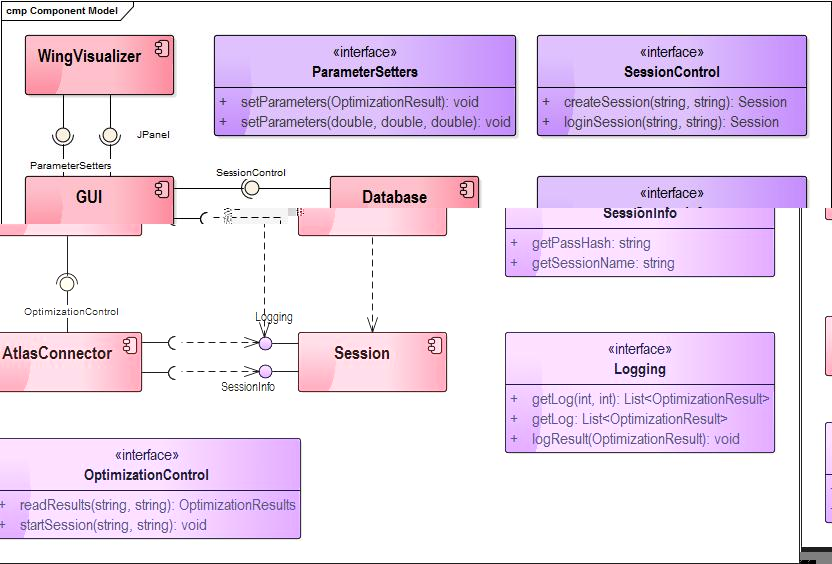
\includegraphics[width=\textwidth]{CompModel.jpg}
\caption{Component diagram}
\end{figure}
\pagebreak

\subsection{Class diagram}
In the following diagram you can see, that the classes in the implemented system are simple reflections of the component design above.
\begin{figure}[h!]
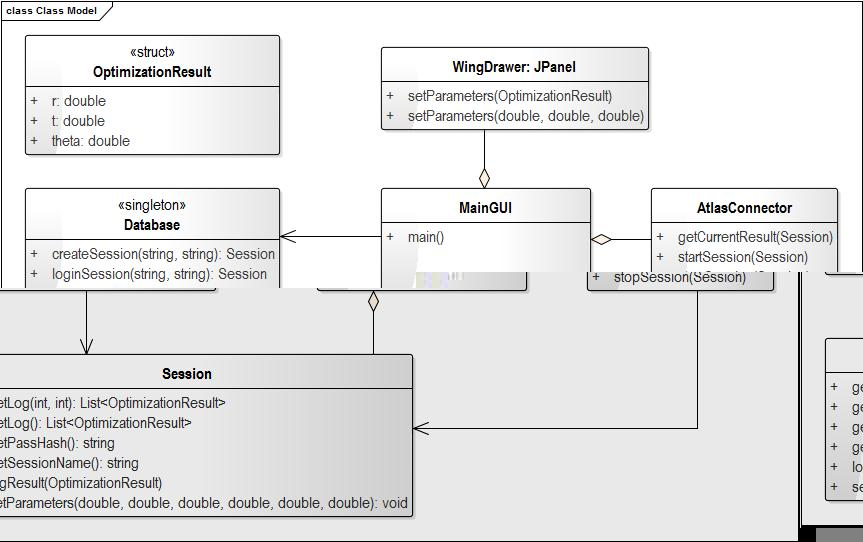
\includegraphics[width=\textwidth]{ClassModel.jpg}
\caption{Class diagram}
\end{figure}
\pagebreak
\subsection{Sequence diagram}
To complement the static diagrams above here we provide a diagram to show the dynamic behaviour of the system. This is not an exact sequence diagram but it shows the flow of data through the system.
\begin{figure}[h!]
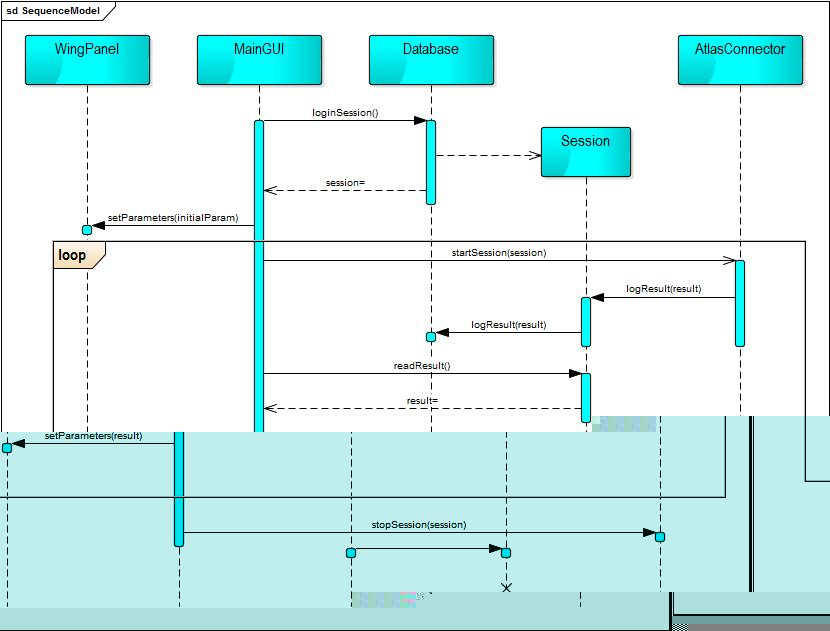
\includegraphics[width=\textwidth]{SequenceModel.jpg}
\caption{Sequence diagram}
\end{figure}

\chapter{Failure case studies}
In this chapter we are going to write about the various failures that can occur during execution of the program and the way they can be avoided or repaired.

\section{Communication errors}
For a system that uses external connections to transfer data between components (like a network) is bound to have some communication errors in time. These can be disconnection issues, data corruption, security issues. As programmers we have to ensure that the system will properly handle these issues without too much data loss.

Failure to do so will lead to the waste of significant computation effort, which can be ultimately translated to the loss of money and time. To avoid or to be prepared for these cases the following measures were taken.

\subsection{Disconnection}
If a network connection disconnects it is only allowed to lose the data being sent, nothing more. For this, proper and thorough logging system needs to be implemented. In our case it is client and server side logging as well.

\subsection{Server side logging}
On the server side simple log files are created. Every line contains the best solution at that point in time. The solution contains the angle of attack, the camber size relative to the chord and the thickness of the wing relative to the chord. The solution also contains the computed the dimensionless values of the lift and drag forces and the ratio of the two for easier data readability. The help the finding of data on the server the log files are named after the session name.

\subsection{Client side logging}
The sessions and the computed values are also logged on the client side of the application. These data are stored in the SQLite database file attached to the program. From that any computation session and it's result can be restored and even continued if the computation didn't finish.

\subsection{Transfer error}
If the messages between the server and the client side get corrupted for any kind of reason, the messages will get discarded, and user will get a notification about possible communication error. The computation will continue and produce relevant data on the server side. If the data in between is not relevant the results can be gathered from the server log, if they are relevant as well, the computation can continue from the last correct message.

\subsection{SSH related errors}
Before the computation could start the program needs to copy the computing part of the program to the remote machine. During these communications errors can occur either with the connection itself, or with the SSH protocol. Later errors include SSH server downtime, user authentication errors etc. Dealing with these issues is outside of the scope of our program, although the program will do anything so that no data should get lost. The program will notify the users about SSH errors, and computation won't start until such issues are handled.

\section{Database error}


\section{Software error}
\subsection{Server side error}
\subsection{Client side error}

\chapter{Conclusion}

\begin{flushleft}
	\bibliographystyle{newapa}
	\bibliography{bibliography}
	\addcontentsline{toc}{chapter}{References}
\end{flushleft}

\end{document}